\documentclass[a4paper,10pt]{report}

\topmargin -2cm
%\topskip0cm
%\footskip0cm
%\headsep0cm
\parindent0cm
\oddsidemargin -1cm
\evensidemargin -1cm
\headheight 2cm
\textheight 24cm
\textwidth 18cm

\author{Daniel W\"aber (4049590)}
\title{\"Ubung}

\usepackage{ucs}
\usepackage[utf8x]{inputenc}
\usepackage{german}
\usepackage{color}
\usepackage{url}
\usepackage{graphicx}
\usepackage{algorithmic}

\pagestyle{empty}
\usepackage{makeidx}
\usepackage{amsmath}
\usepackage{amsfonts}
\usepackage{amssymb,euscript}
\usepackage{dsfont}
\usepackage{listings}
\usepackage{enumerate}
\newfont{\Fr}{eufm10}
\newfont{\Sc}{eusm10}
\newfont{\Bb}{msbm10}
\newcommand{\limin}{\lim_{n\rightarrow\infty}}
\newcommand{\limix}{\lim_{x\rightarrow\infty}}
\newcommand{\limun}{\lim_{n\rightarrow -\infty}}
\newcommand{\limux}{\lim_{n\rightarrow -\infty}}
\newcommand{\limx}{\lim_{x\rightarrow x_0}}
\newcommand{\limh}{\lim_{h\rightarrow 0}}
\newcommand{\defi}{\paragraph{Definition:}}
\newcommand{\bew}{\paragraph{Beweis:}}
\newcommand{\satz}{\paragraph{Satz:}}
\newcommand{\bsp}{\paragraph{Beispiel:}}
\newcommand{\lemma}{\paragraph{Lemma:}}
\newcommand{\N}{\mathds{N}}
\newcommand{\F}{\mathds{F}}
\newcommand{\Z}{\mathds{Z}}
\newcommand{\Q}{\mathds{Q}}
\newcommand{\R}{\mathds{R}}
\newcommand{\G}{\mathds{G}}
\newcommand{\C}{\mathds{C}}
\newcommand{\K}{\mathds{K}}
\newcommand{\A}{\mathds{A}}
\newcommand{\E}{\mathcal{E}}
\renewcommand{\P}{\mathcal{P}}
\newcommand{\sigA}{$\sigma$-Algebra }
\newcommand{\qed}{$\hfill\blacksquare$}
\newcommand{\arsinh}{\operatorname{arsinh} }
\newcommand{\arcosh}{\operatorname{arcosh} }
\newcommand{\gdw}{ $ \Leftrightarrow $ }
\newcommand{\tf}{ $ \Rightarrow $ }
\newcommand{\mgdw}{\Leftrightarrow}
\newcommand{\mtf}{\Rightarrow}
\newcommand{\Bild}{\text{Bild}}
\newcommand{\Kern}{\text{kern}}
\newcommand{\rg}{\text{rg}}
\newcommand{\deff}{\text{deff}}

\newcommand{\alphato}{\underset{\alpha}\to}
\newcommand{\betato}{\underset{\beta}\to}
\newcommand{\etato}{\underset{\eta}\to}
\newcommand{\ito}{\underset{i}\to}
\newcommand{\sto}{\underset{s}\to}
\newcommand{\kto}{\underset{k}\to}
\newcommand{\xto}{\underset{x}\to}

\usepackage{fancyhdr}
\pagestyle{fancy}
\lhead{Daniel Waeber\\Alex Muenn}
\chead{"Ubungsblatt \nr\\\today}
\rhead{Bildverarbeitung}


\newcommand{\nr}{2}
\lstset{language=matlab}

\begin{document}
\section*{Aufgabe 1 - 2D Konvolution}
F\"ur die Realisierung der Konvolution haben wir die Funktionen aus der
vorherigen \"Ubung verwendet, die lediglich die Operation 
$F^{-1}(F*K*F .* F*B*F)F^{-1}$ mit Hilfe der FFT ausf\"uhrt.
\\
Hauptaufgabe bestand hierbei in dieser Aufgabe in der korrekten  Konstruktion 
der Faltungsmatrizen (als Kernel $K$). Wobei $K$ mit dem Bild konvolviert wird und
anschaulich mit dem ersten Element $K(1,1)$ \"uber das Bild ``f\"ahrt''. Daraus
ergibt sich, dass der Mittelpunkt der geforderten Kernel in der linken oberen Ecke
liegen m\"ussen und die \"Uberh\"ange an die entsprechenden R\"ander/Ecken der Matrix
geshiftet werden m\"ussen. Die Konvolution setzt diese Ecken zwangsl\"aufig wieder
korrekt zusammen.

\subsection*{Generierung der Kernel}
\begin{enumerate}
\item Gauss 3\&10: Erstellung einer $NxN$ Matrix, Anwendung der Gaussfunktion 
      in 2D mit Parametern $\varsigma$ und $x, y$, f\"uhrt zu zentriertem Auge $ \to $ shiften
\item Sobel X: $ \begin{pmatrix} 1 & 0 & -1 \\ 2 & 0 & -2 \\ 1 & 0 & -1  \end{pmatrix}$ einf\"ugen
in zeros $NxN$ und wieder shift nach links und nach oben
\item Sobel Y: $-1 Sx^{T}$
\item Uniform: $1/25*(5x5\text{matrix})$ \ldots analog zu den vorherigen
\end{enumerate}

\subsection*{Beobachtung}
Bei allen Kerneln ``Artefakte'' an den R\"andern (durch Faltung mit \"uberliegender Kante)
\begin{enumerate}
\item Gauss(3): relativ starkes Weichzeichen
\item Gauss(10): nahezu unerkenntliche Weichzeichnung
\item Sobel X: Da Ableitung in X Richtung, werden starke Frequenz\"uberg\"ange in X Richtung
erkannt, also Kanten die senkrecht im Bild verlaufen. Hier speziell die Haare und einzelnen 
Partien im Gesicht und eine Kante im Hintergrund
\item Sobel Y: \"ahnlich zu Sobel X nur hier die waagerechten Kanten, auch Gesicht (Augen!) und
liegenden Haare
\item uni: Weichzeichnung \"ahnlich zu Gauss, allerdings blieben hier die Kontraste erhalten
\end{enumerate}

\section*{Aufgabe 2 - 2D Dekonvolution}
Weil der Kernel bekannt ist, kann das Originalbild durch Umformung der Konvolutionsgleichung
wieder hergestellt werden: $B_{deconv}=F^{-1}*(FB_{conv}F ./ FKF)*F^{=1}$
\\
Ein Problem entsteht hier allerdings sobald in der transformierten Kernel-Matrix Elemente mit
dem Wert $0$ stehen. Diese haben wir ``provisorisch'' durch sehr kleine Werte ersetzt. 
Alle Originalbilder liessen sich ohne sichtlichen Unterschied wieder rekonstruieren.

\section*{Aufgabe 3 - 2D Dekonvolution nach Rauschen}
Auf alle konvolvierten Bilder addierten wir eine Matrix gleicher Gr\"osse, wie gefordert, mit
gaussschem Rauschen.
\\
Zum einen l\"asst sich beobachten, dass das Rauschen die Rekonstruktion zunehmend
verschlechtert, je gr\"osser der Bereich des Kernels ist. Gauss10 sieht erheblich schlechter
aus als Gauss3, der jedoch wiederum auch schlechter gegen\"uber der uniformen (De)Konvolution
da steht. Zum anderen lassen sich anhand der verrauschten Rekonstruktion ebenfalls R\"uckschl\"usse auf den Kernel ziehen. Bei den Sobel Kerneln entsehen zus\"atzliche Streifen, analog
ihrer Orientierung, die uniforme Dekonvolution fuehrt zu einem Krisselmuster und bei Gauss'schen Verfahren ver\"andert sich zus\"atzlich der Farbwert (das Bild erscheint eher Schwarz-Weiss als in Grauwerten).

\section*{Ausgaben}
Alle Bilder haben 
\begin{figure}[H]
\begin{center}
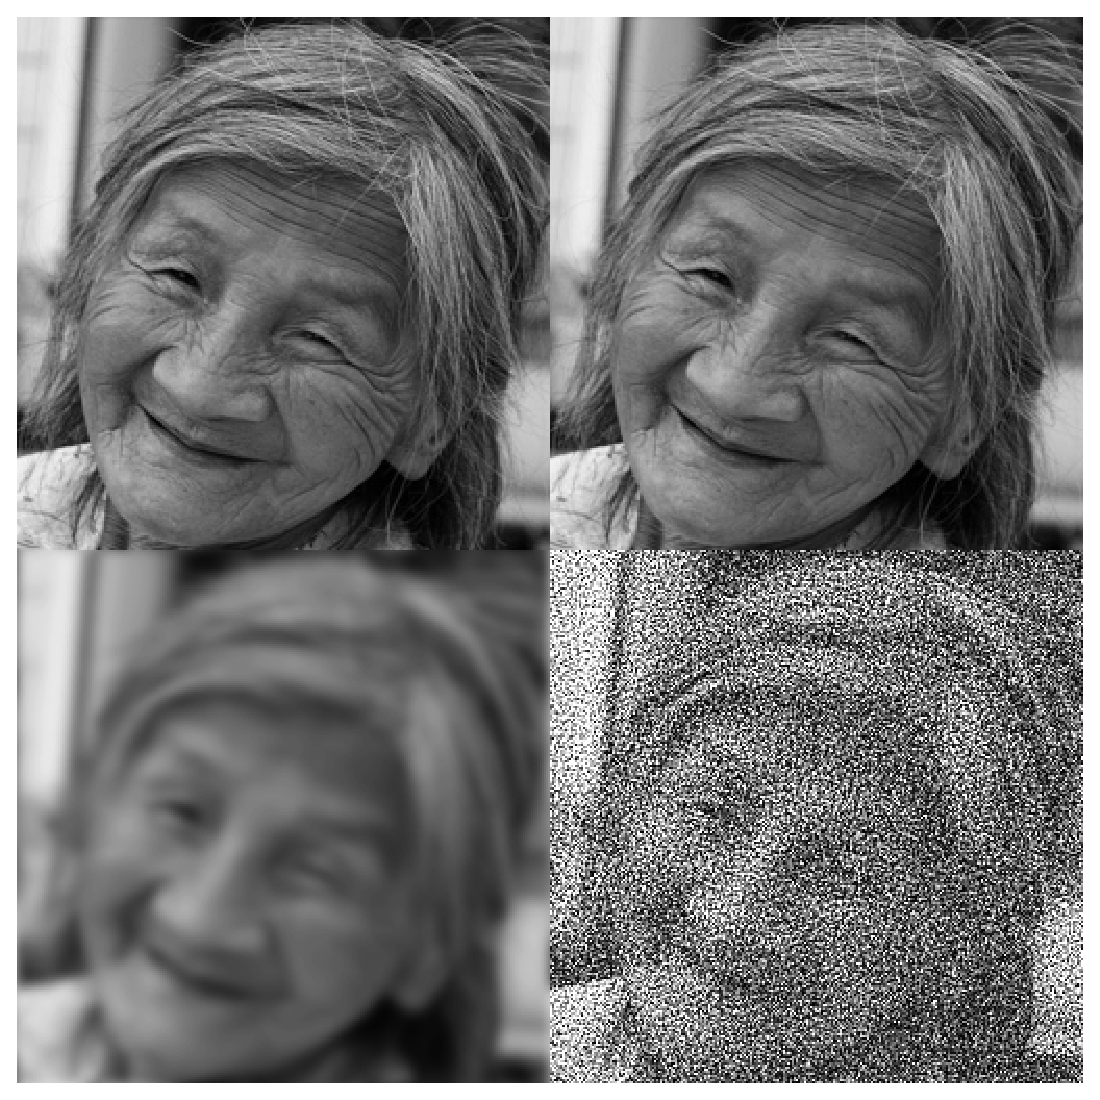
\includegraphics[width=100mm]{u03/gauss_3.eps}
\end{center}
\caption{Gauss3}
\end{figure}

\begin{figure}[H]
\begin{center}
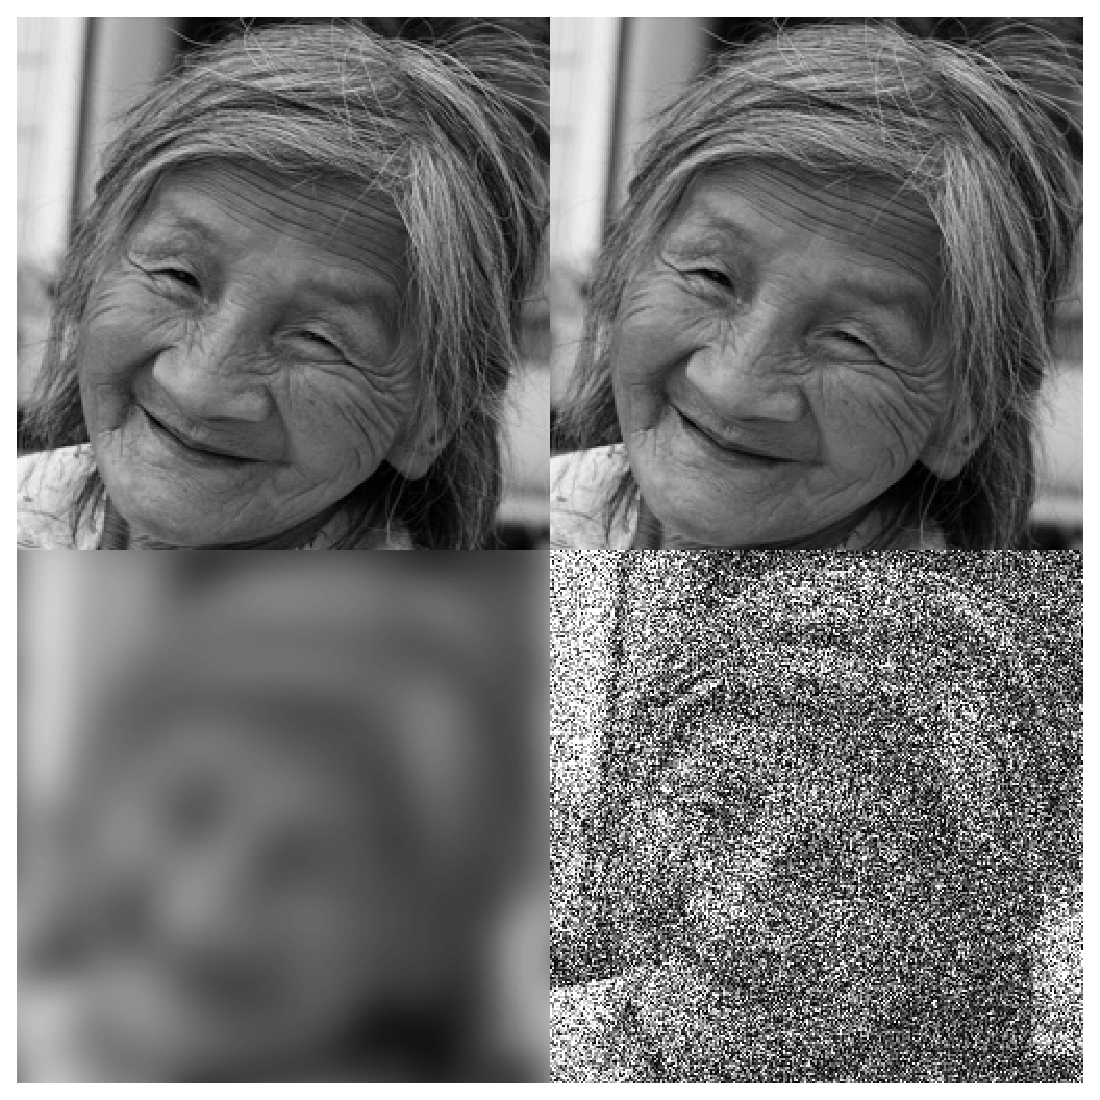
\includegraphics[width=100mm]{u03/gauss_10.eps}
\end{center}
\caption{Gauss10}
\end{figure}

\begin{figure}[H]
\begin{center}
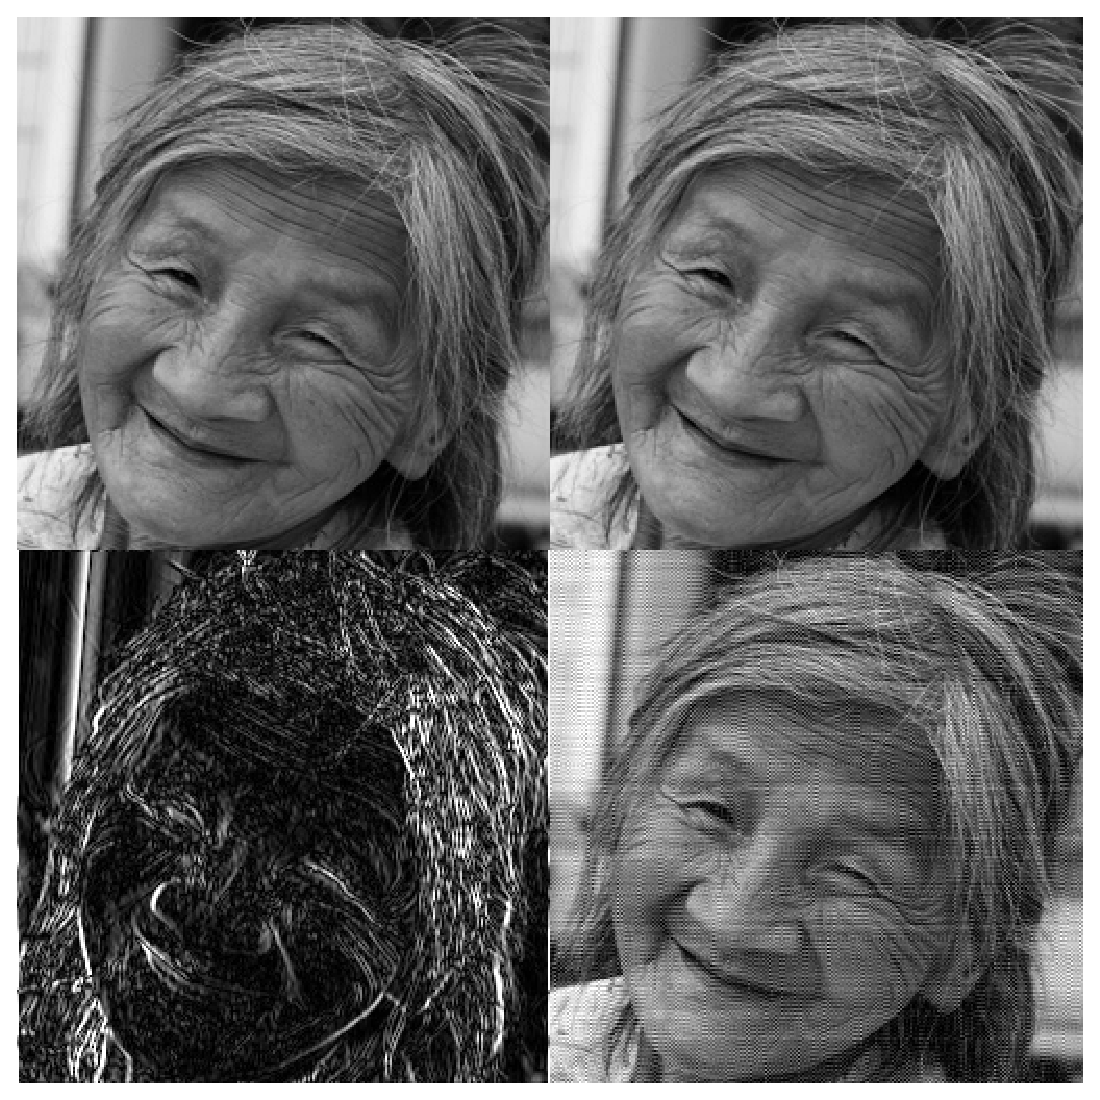
\includegraphics[width=100mm]{u03/sobel_x.eps}
\end{center}
\caption{Sobel X}
\end{figure}

\begin{figure}[H]
\begin{center}
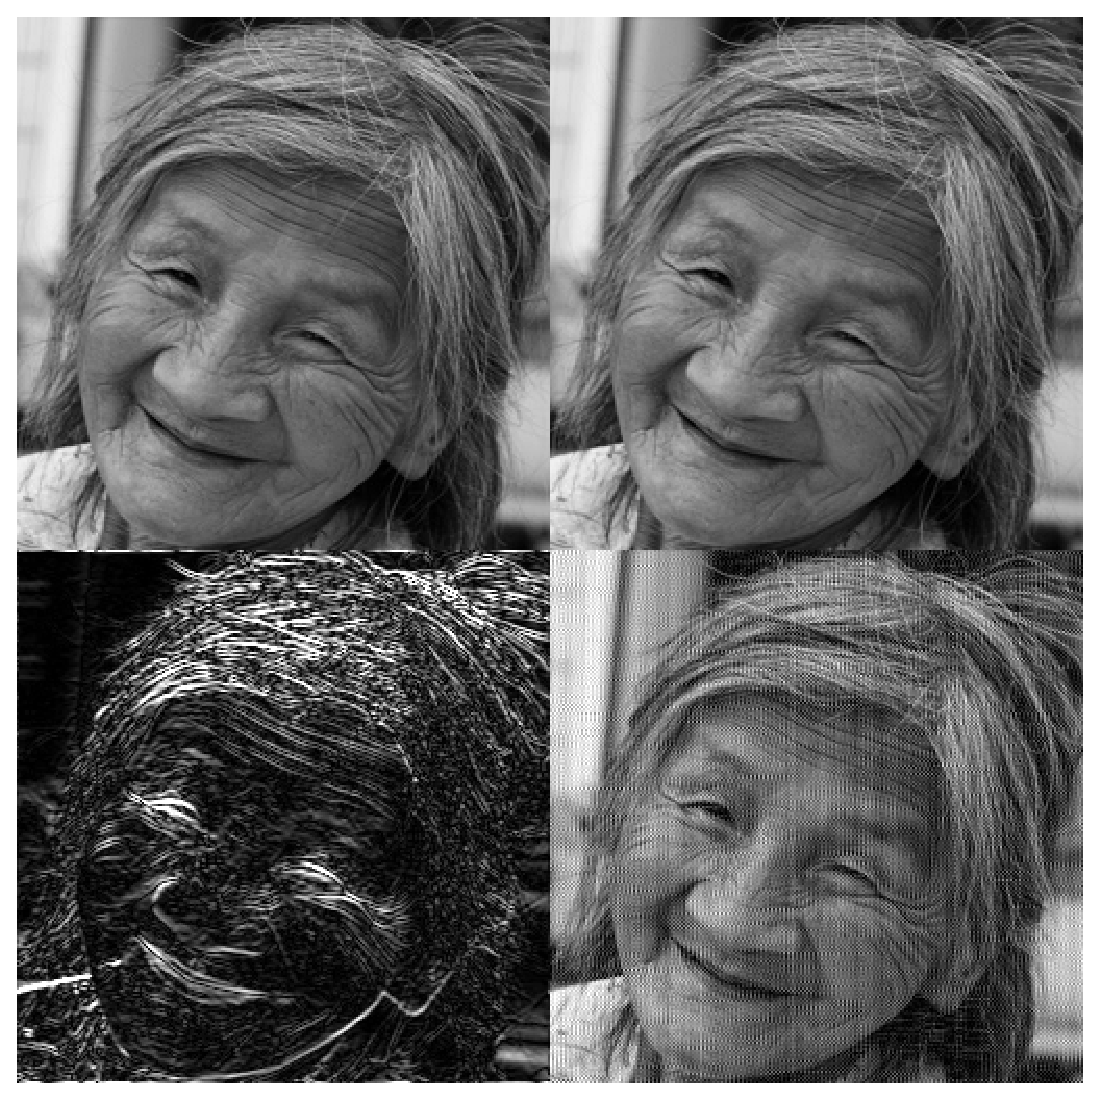
\includegraphics[width=100mm]{u03/sobel_y.eps}
\end{center}
\caption{Sobel Y}
\end{figure}

\begin{figure}[H]
\begin{center}
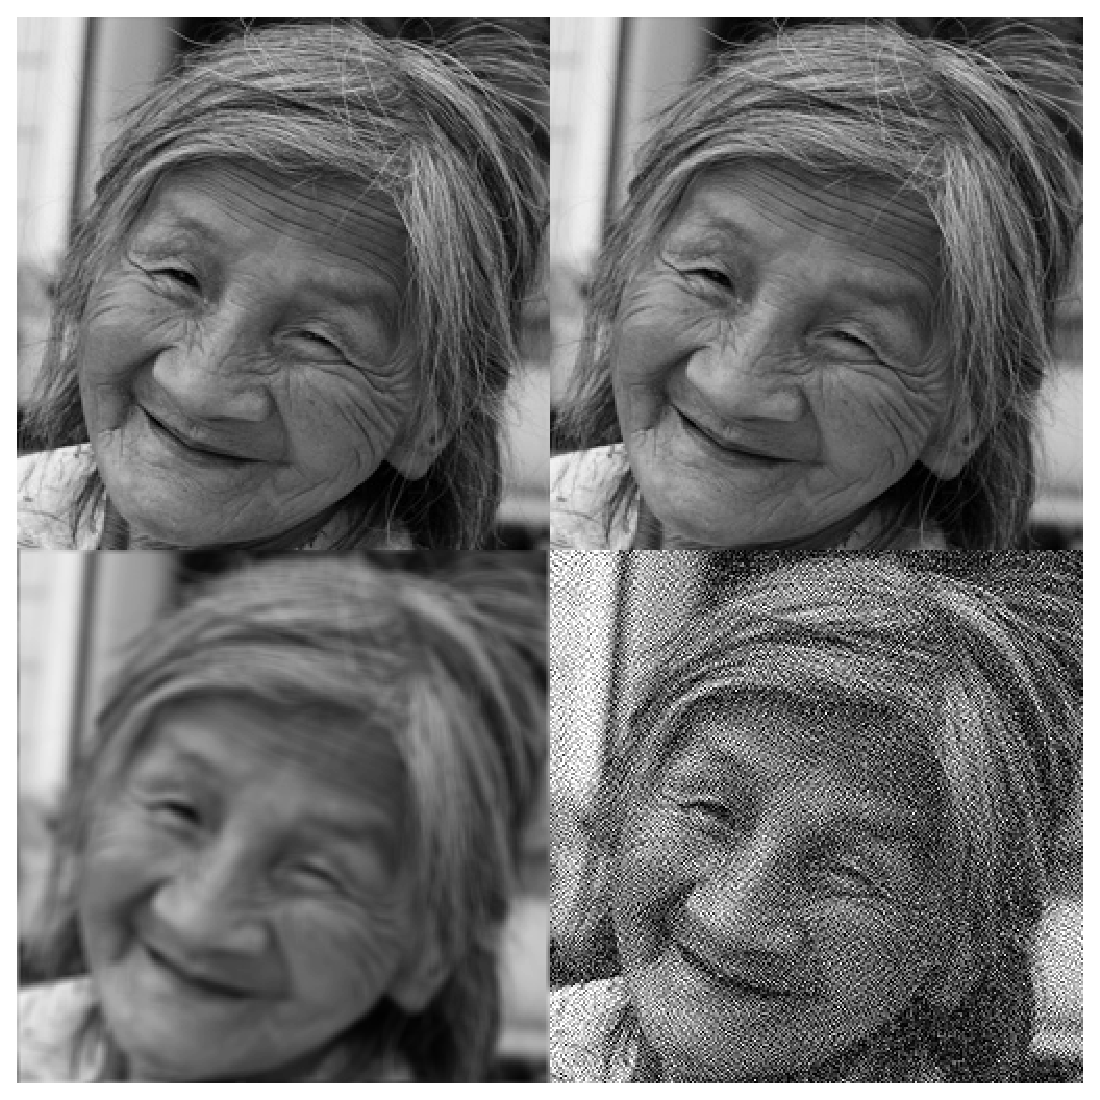
\includegraphics[width=100mm]{u03/uni.eps}
\end{center}
\caption{Uniform}
\end{figure}

\end{document}
